%!TEX root = ../thesis.tex


% FIGURE: Mass vs. lifetime
% https://www.sciencedirect.com/science/article/pii/S0146641019300109
\begin{figure*}[p!]
  \centering %\vspace{-6mm}
  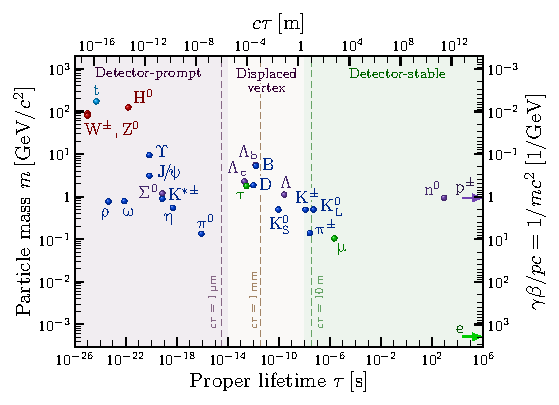
\includegraphics[width=10.5cm]{fig/objects/SM_particles_masses.pdf}
  \vspace{-2mm}
  \caption{
Plot of the mass versus lifetime $\tau$ of many composite and fundamental SM particles.
The particles in the green-shaded region have a lifetime long enough to travel into the detector before decaying.
Particles in the orange-shaded zone can travel some measurable distance, creating a decay vertex measurably displaced from the production vertex, whereas the decay length of those in the purple-shaded region are not observable.
Note that relativistic particles will travel a larger distance on average due to time dilation, with the decay length give by $L=\gamma\beta c\tau$, with $\gamma\beta=p/mc$.
Adapted from~\cite{lifetime_plot}.
  } \label{fig:lifetime}
\end{figure*}